\documentclass[]{article}

\usepackage[nottoc,numbib]{tocbibind}

\usepackage{amssymb,amsmath}
\setcounter{tocdepth}{3}
\usepackage{graphicx}
\usepackage{algorithm, algorithmic}
\usepackage{caption}
\usepackage{complexity}
\usepackage{subcaption}
\usepackage{tabularx}
\usepackage{cite}
\usepackage{pgfgantt}
\graphicspath{{images/}}
\captionsetup{compatibility=false}

%\usepackage{setspace}
%%\singlespacing
%%\onehalfspacing
%\doublespacing

\DeclareMathOperator*{\argmax}{argmax}

\DeclareMathOperator*{\optimise}{optimise}
\DeclareMathOperator*{\subjectto}{subject\hspace{0.1cm}to}
%opening
\title{Evolutionary Optimization of Residential Floor Plans}
\author{Zuxing Wu\\a1816653\\ \\Supervisors: Adel Nikfarjam\\ }

\begin{document}

\maketitle\nonumber

\newpage\nonumber

\tableofcontents

\newpage

% \begin{abstract}
% Abstract
% \end{abstract}
\section{Research Topic Title} 
Evolutionary Optimization of Residential Floor Plans
\section{Research Topic Summary}

Residential floor plan design is a complex and challenging task that requires careful consideration of various factors, such as room sizes, adjacencies, and orientations. Traditional methods of floor plan design are often time-consuming and labor-intensive, leading to suboptimal solutions. Evolutionary algorithms have been proposed as a promising alternative for optimizing floor plans, as they can efficiently explore the design space and generate high-quality solutions. This project aims to develop a new method for optimizing residential floor plans using evolutionary algorithms and address some limitations of previous research. The proposed method will involve the application of evolutionary algorithms to generate and evolve floor plans based on a novel representation scheme. The fitness of each floor plan will be evaluated based on objective criteria (e.g.\ energy consumption) and subjective criteria (e.g.\ privacy, comfort, practicality, convenience). The performance of the proposed method will be evaluated using a set of benchmark problems and compared with existing approaches. The results of this project will contribute to the field of residential floor plan design and provide valuable insights into the application of evolutionary algorithms to architectural design problems.

\section{Introductory Background}
Residential floor plan design is a critical aspect of architectural design that involves the layout of rooms, corridors, and other spaces within a building. The design of a floor plan can have a significant impact on the functionality, aesthetics, comfort, ventilation and energy efficiency of a building. Traditional methods of floor plan design are often based on manual sketches or computer-aided design (CAD) tools, which can be time-consuming and labor-intensive. Moreover, these methods may not always produce optimal solutions, as they rely on the intuition and experience of the designer.

Evolutionary algorithms have been proposed as a promising alternative for optimizing floor plans, as they can efficiently explore the design space and generate high-quality solutions. Evolutionary algorithms are a class of optimization algorithms inspired by the process of natural selection. They work by maintaining a population of candidate solutions (individuals) and iteratively applying genetic operators (e.g.\ crossover, mutation) to generate new solutions. The fitness of each solution is evaluated based on a predefined fitness function, which measures how well the solution satisfies the objectives of the optimization problems.

\section{Literature Review}
Previous research has explored the application of evolutionary algorithms to optimize residential floor plans. Brintrup et al.~\cite{10.1007/11732242_56} compared 3 interactive genetic algorithms (i.e.\ sequential IGA, multi-objective IGA, parallel IGA) on a multi-objective floor planning task, and found the multi-objective IGA provides more diverse results and faster convergence for optimizing floor plan. It was found that proportional roulette wheel selection is the best parent selection method for the mating pool, and k-point crossover is the most effective for fitness evolutionary improvement~\cite{7844659}.

Combining Evolutionary algorithm with Greedy-like algorithm can help find the near-optimal solution in Automated Floor Plan Generation (AFPG) though it is a simplified model of multi-objective optimization by linear composition of the partial evaluation functions~\cite{doi:10.1177/1478077119832982}. Subramanian et al.~\cite{9675541} used Genetic Algorithm with KD tree models in a web application to generate floor plans for even non-expert users.

Wang and Duan~\cite{WANG2023100238} tried to optimize the floor plan design by focusing on the energy consumption and consumer satisfaction, which proves that the preferences of different types of consumers differed significantly. Therefore, different evaluation criteria are needed for satisfying different family types~\cite{WANG2023100238}. The quality and efficiency of residential floor plan design can be improved by combining Monte Carlo tree search algorithm (MCTS) and particle swarm optimization (PSO)~\cite{YAN2024110546}. The MCTS algorithm takes human experience into consideration so that it can compress the search space and simplify the solution process~\cite{YAN2024110546}. Meanwhile, the PSO algorithm can increase the search speed and efficiency owing to its parallel processing ability~\cite{YAN2024110546}.

Enengy consumption, probable uniformity (PU), and spatial useful daylight illuminance (sUDI) are three objectives that are considered in the optimization process using NSGA-II algorithm, and the results show that the NSGA-II algorithm can provide a set of more sustainable floor plans requiring less computational power and time~\cite{CHAICHI2024108842}.

\section{Aims, Objectives of the Project}
This project aims to develop a new and efficient method for optimizing residential floor plans using evolutionary algorithms, and address some limitations of previous research.
The main objectives of this project are as follows: 
\begin{itemize}
    \item Implement an efficient initialization strategy for the generation of the initial population.
    \item Develop a more robust evolutionary optimization framework tailored to residential floor plans.
    \item Propose a novel representation scheme for residential floor plan layouts.
    \item Conduct a comprehensive comparison of the proposed method with existing approaches to evaluate its performance.
\end{itemize}

\section{Methodology}
The methodology of this project involves the application of evolutionary algorithms to optimize residential floor plans. The process will be divided into several key stages: initialization of the population, representation of the floor plan, design of the evolutionary optimization framework, and performance evaluation. These stages are outlined below.

\subsection{Population Initialization}
The first step in the evolutionary process is to generate an initial population of residential floor plans. An efficient initialization strategy will be employed to ensure diversity within the population while adhering to basic architectural constraints, such as room adjacency and size. Specifically, it contains 2 stages: 1. Locate room positions, 2. Locate wall positions based on room sizes~\cite{10.1145/3355089.3356556}.

\subsection{Representation of Floor Plans}
Residential floor plans will be represented using a novel structure, parse tree~\cite{khade2023}, that encodes the spatial relationships between rooms, such as adjacency and sizes. The representation will be designed to allow for easy manipulation by evolutionary operators (e.g.~crossover and mutation) while preserving architectural feasibility and obeying relevant constraints.

\subsection{Evolutionary Optimization Framework}
The evolutionary optimization framework will be based on a standard evolutionary algorithm, with modifications to better suit the characteristics of floor plan design. The selection process will prioritize diversity to avoid premature convergence, while the crossover operator will combine features of two or more floor plans to produce offspring with novel characteristics. Mutation will introduce small random changes to further explore the design space. The fitness of each floor plan will be evaluated based on objective criteria (e.g.\ energy consumption), subjective criterion (e.g.\ privacy, comfort, practicality, convenience), and compliance with architectural standards. If necesssary, more than one evolutionary algorithm will be used in the process of optimizing the floor plan. For example, Monte Carlo tree search algorithm (MCTS) handles discrete variables and particle swarm optmization (PSO) deals with continuous variables~\cite{YAN2024110546}.

\subsection{Fitness Function Design}
The fitness function will evaluate each floor plan based on several criteria:
1. Objective criteria: energy consumption.
2. Subjective criteria: privacy, comfort, practicality, convenience.
The energy performance evaluation can be achieved by simulation in Topologic~\cite{WANG2023100238}. The subjective criteria can be evaluated by a group of human evaluators, shown as Table~\ref{table1}.
\begin{table}[h]
  \centering
  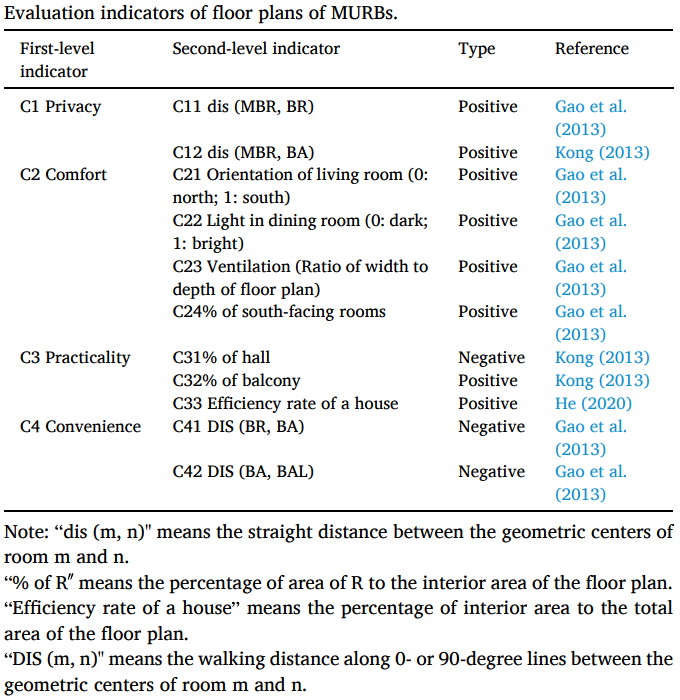
\includegraphics[width=0.8\textwidth]{image1.png}
  \caption{Evaluation indicators. Table 2 of Wang and Duan\cite{WANG2023100238}}\label{table1}
\end{table}

The straight distance between the geometric centers of room $m$ and $n$ is defined as:
\begin{equation*}
\text{dis}(m, n) = \sqrt{(x_m - x_n)^2 + (y_m - y_n)^2}
\end{equation*}

The percentage of area of $R$ to the interior area of the floor plan is defined as:
\begin{equation*}
\% \text{ of } R = \left( \frac{\text{Area of } R}{\text{Interior Area of Floor Plan}} \right) \times 100\%
\end{equation*}

The efficiency rate of a house is defined as the percentage of interior area to the total area of the floor plan:
\begin{equation*}
\text{Efficiency Rate} = \left( \frac{\text{Interior Area}}{\text{Total Area}} \right) \times 100\%
\end{equation*}

The walking distance along 0- or 90-degree lines between the geometric centers of room $m$ and $n$ is defined as:
\begin{equation*}
\text{DIS}(m, n) = |x_m - x_n| + |y_m - y_n|
\end{equation*}


The proposed method will be implemented in Python. The optimization process will be carried out in two stages: initialization and evolution. The initialization stage will involve generating an initial population of floor plans using a novel strategy. The evolution stage will consist of iteratively applying genetic operators to the population to produce new generations. The fitness of each individual will be evaluated using a fitness function that considers various factors such as the number of rooms, room sizes, and room adjacencies. The optimization process will be repeated for a specified number of generations or until a termination criterion is met. The performance of the proposed method will be evaluated using a set of benchmark problems and compared with existing approaches.

\section{Significance}
The proposed research method will contribute to the field of residential floor plan design by providing a new and efficient approach to optimizing floor plans using evolutionary algorithms. The method will address some limitations of previous research and offer valuable insights into the application of evolutionary algorithms to architectural design problems. The results of this project will be of interest to architects, designers, and researchers working in the field of architectural design and optimization. The proposed method has the potential to improve the quality, diversity and efficiency of residential floor plan design and lead to the development of innovative and sustainable building designs.

\section{Research Plan}
My research plan consists of four main phases:
\begin{itemize}
  \item Phase 1
    \begin{enumerate}
      \item Population initialization
  \item Solution representation
    \end{enumerate}
  \item Phase 2
  \begin{enumerate}
    \item Evolutionary optimization
    \item Solution evaluation
  \end{enumerate}
\end{itemize}
Each phase will involve specific tasks and activities that will be carried out over a period of 6 months. The timeline for the research plan is shown in the Gantt chart below. \\
\begin{ganttchart}[
  hgrid,
  vgrid,
  x unit = 1.4cm,
  y unit chart=0.7cm,
  title/.append style={fill=none},
  title label font=\bfseries\footnotesize,
  title label anchor/.append style={below=-1.6ex},
  include title in canvas=false,
  bar label font=\normalsize\scshape,
  bar label node/.append style={left=2ex},
  bar/.append style={fill=yellow!60},
  group/.append style={fill=cyan!80},
  bar incomplete/.append style={fill=red!30},
  progress label text={},
  group right shift=0,
  group top shift=0.7,
  group height=.3
]{1}{6}
\gantttitle{2024.09--2025.02}{6} \\
\gantttitlelist{9,10,11,12,1,2}{1} \\
\ganttgroup{Phase 1}{1}{3} \\
\ganttbar{Initialization}{1}{2} \\
\ganttbar{Representation}{2}{3} \\
\ganttgroup{Phase 2}{4}{6} \\
\ganttbar{Optimization}{4}{5} \\
\ganttbar{Evaluation}{5}{6} \\
\end{ganttchart}

\section{Plagiarism Declaration}
I hereby declare that this submission is my own work and to the best of my knowledge, it contains no material previously published or written by another person, except where due to acknowledgment is made. Furthermore, I believe that it contains no material which has been accepted for the award of other degree or diploma in any university or other tertiary institutions.


\bibliographystyle{abbrv}
\bibliography{MyReferences}

\end{document}

